\documentclass{beamer}
\usetheme{Warsaw}

\usepackage[utf8]{inputenc}
\usepackage{fancybox}
\usepackage{multimedia} 
\usepackage{subfig}
\usepackage{amsmath}
\usepackage{hyperref}
\usepackage[all]{xy}
\usepackage{algorithm}
%\usepackage{arevmath}     % For math symbols
\usepackage[noend]{algpseudocode}

\begin{document}


\title[Angewandte Mathematik] % (optional, only for long titles)
{Angewandte Mathematik
\\
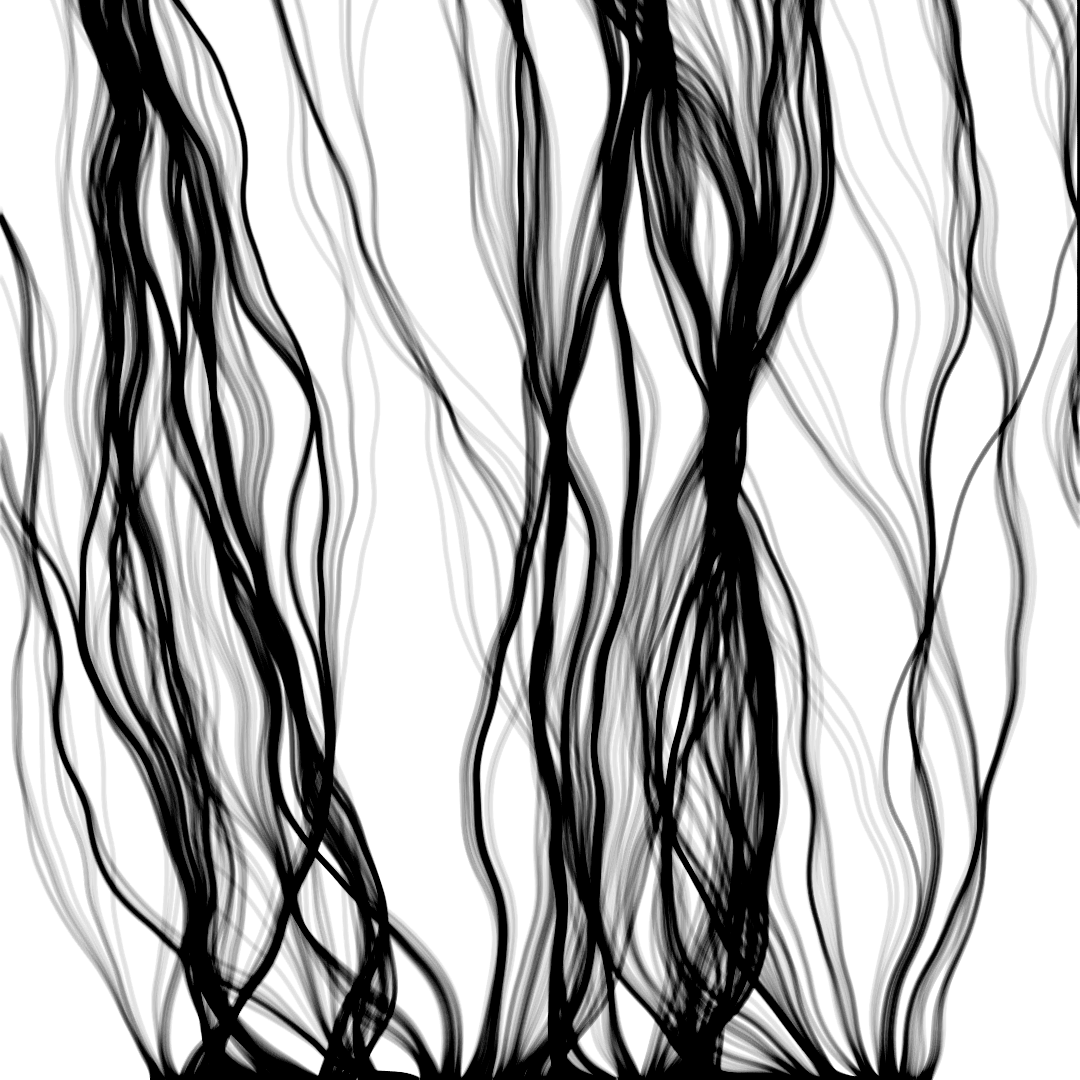
\includegraphics[scale=0.15]{images/cover}
}
\subtitle{}
\author[Dr. Johannes Riesterer] % (optional, for multiple authors)
{Dr.  rer. nat. Johannes Riesterer}

\date[KPT 2004] % (optional)
{}

\subject{Angewandte Mathematik}



\frame{\titlepage}



\begin{frame}
    \frametitle{Angewandte Mathematik}
\framesubtitle{Lebesgue Integral}
\begin{block}{Schnittmenge}
Sei $ A \subset \mathbb{R}^n$. Für $ y \in \mathbb{R}^p$ heißt
$$ A_y :=  \biggl \{    x \in \mathbb{R}^{n-p}  \; | \;  (x,y) \in A \biggr \}$$  
Schnittmenge von $A$ zu $y$.
\end{block}
 \end{frame}



\begin{frame}
    \frametitle{Angewandte Mathematik}
\framesubtitle{Lebesgue Integral}
\begin{block}{Kleiner Satz von Fubini}
Sei $A \subset \mathbb{R}^n$ eine offene und beschränkte Teilmenge und $f : U \to \mathbb{R}$  eine stetige und beschränkte Funktion.
Dann ist für jedes $ y \in \mathbb{R}^p$ mit $A_y \neq \emptyset$ die Funktion $f_y(x) := f(x,y)$ über $A_y$ und   
$$ F(y) := \begin{cases}   \int_{A_y} f(x,y) d \mu_{p}  , \text{ falls }  A_y \neq \emptyset 
\\ 0 \text{ sonst } \end{cases} $$
über $\mathbb{R}^{p}$ integrierbar und es gilt 
$$ \int_A f(x,y) d \mu_n = \int_{\mathbb{R}^p } F(y) d \mu_p \; .$$
 Hierfür schreiben wir auch kurz
$$ \int_A f(x,y) d \mu_n  = \int_{\mathbb{R}^{p} }  \biggl ( \int_{A_y} f(x,y)  d\mu_{n-p} \biggr ) d\mu_p$$
\end{block}
 \end{frame}



\begin{frame}
    \frametitle{Angewandte Mathematik}
\framesubtitle{Beweis}
Sei  $\varphi_k$ eine monoton wachsende Folge von Treppenfunktionen auf $\mathbb{R}^n$ mit $|| f_A - \varphi_k ||_1 \to 0$.
Für jedes $y \in \mathbb{R}^p$ bilden dann die Funktionen $\varphi_k(x)_y := \varphi_k(x,y)$ eine monoton wachsende Folge von Treppenfunktionen auf $\mathbb{R}^{n-p}$, die gegen $f_y(x):= f_A(x,y)$ konvergiert. Die Folge der Integrale $\int_{\mathbb{R}^{n-p}} \varphi_k(x)_y d \mu_{n-p}$ ist beschränkt,  da $A$ beschränkt ist, und daher gibt es eine Quader $I$ mit $U \subset I$ und  mit $M : = \max (f)$  ist $\int \varphi_k d \mu \leq M \mu(I)$ beschränkt. Mit dem kleinen Satz von B. Levi
gilt
$$ F(y) := \lim_{k \to \infty} \int_{\mathbb{R}^{n-p}} \varphi_k(x)_y d \mu_{n-p} \; .$$
 \end{frame}



\begin{frame}
    \frametitle{Angewandte Mathematik}
\framesubtitle{Beweis}
Die Funktionen 
$$\phi_k (y) := \int_{\mathbb{R}^{n-p}} \varphi_k (x,y) d \mu_{n-p}$$
sind Treppenfunktionen auf $\mathbb{R}^{p}$ und die Folge $\phi_k$ konvergiert monoton wachsend gegen $F$ und die Folge der Integrale 
$\int \phi_k(y) d \mu_{p}$ ist beschränkt, da  mit dem Satz von Fubini für Treppenfunktionen und $\varphi_k \leq f_A$  
$$ \int_{\mathbb{R}^{p}} \phi_k(y) d \mu_{p} = \int_{\mathbb{R}^n} \varphi_k(x,y) d\mu_{n} \leq \int_{\mathbb{R}^n} f_A(x,y) d \mu_{n} \; .$$
Mit dem kleinen Satz von B. Levi ist $F$ integrierbar und es gilt
\begin{align*}
 \int_{\mathbb{R}^{p}}   F(y) d \mu_{p} & = \lim_{k \to \infty}  \int_{\mathbb{R}^{p}}  \phi_k (y) d \mu_{p} =  \lim_{k \to \infty}  \int_{\mathbb{R}^{n}}  \varphi_k(x,y) d \mu_{n} \\
& =   \int_{\mathbb{R}^{n}}  f_A (x,y) d \mu_{n}  \; .
\end{align*} 

 \end{frame}




\begin{frame}
    \frametitle{Angewandte Mathematik}
\framesubtitle{Lebesgue Integral}
\begin{block}{Riemann vs. Lebesgue}
Eine \href{https://de.wikipedia.org/wiki/Regelfunktion}{Regelfunktion} $f$ auf $[a,b] \subset \mathbb{R}$ ist über $[a,b] $ Lebesgueintegrierbar und es gilt 
\begin{align*}
\int_{[a,b]} f(x) d \mu_1 = \int_a^b f(x) dx \; .
\end{align*}
\end{block}
 \end{frame}






\begin{frame}
    \frametitle{Angewandte Mathematik}
\framesubtitle{Beweis}
Sei $\varphi_k$ eine Folge von Treppenfunktionen mit $|| f -\varphi_k ||_{\infty} \to 0$. Da für jede Funktion $h$ auf $[a,b]$ die Abschätzung
$|h| \leq || h ||_{\infty} 1_{[a,b]}$ gilt, folgt auch $$|| f_A -\varphi_{k,A} ||_{1} \to 0$$ und damit ist $f_{[a,b]}$ auch Lebesgueintegrierbar über $[a,b]$ mit Lebesgueintegral
\begin{align*}
\int_{[a,b]} f(x) d \mu= \int_{\mathbb{R}} f_A(x) d\mu = \lim_k \int_{\mathbb{R}} \varphi_{k,A} d \mu = \lim_k \int_a^b \varphi_k dx = \int_a^b f (x) dx
\end{align*}
 

 \end{frame}



\begin{frame}
    \frametitle{Angewandte Mathematik}
\framesubtitle{Lebesgue Integral}
\begin{block}{Beispiel}
Sei $K := B^2_1(0) := \{   (x,y) \in \mathbb{R}^2 \; | \; \sqrt{x^2 + y^2 } \leq 1\}$. Mit dem kleinen Satz von Fubini erhalten wir
\begin{align*}
\int_K 1 d \mu = &  \int_{-1}^{1} \biggl ( \int_{-\sqrt{1- y^2}}^{\sqrt{1- y^2}} 1 dx \biggr ) dy = \\ 
& =  2 \int_{-1}^{1}  \sqrt{1 - y^2}   \; dy  \\ 
 & (substitution \;   y = sin(u)) =   2 \int_{-\frac{\pi}{2}}^{\frac{\pi}{2}}   \cos(u)^2   \; du = 2 \cdot \frac{\pi}{2} = \pi
\end{align*}
\end{block}
 \end{frame}



\begin{frame}
    \frametitle{Angewandte Mathematik}
\framesubtitle{Lebesgue Integral}
\begin{figure}[H]
      \centering
    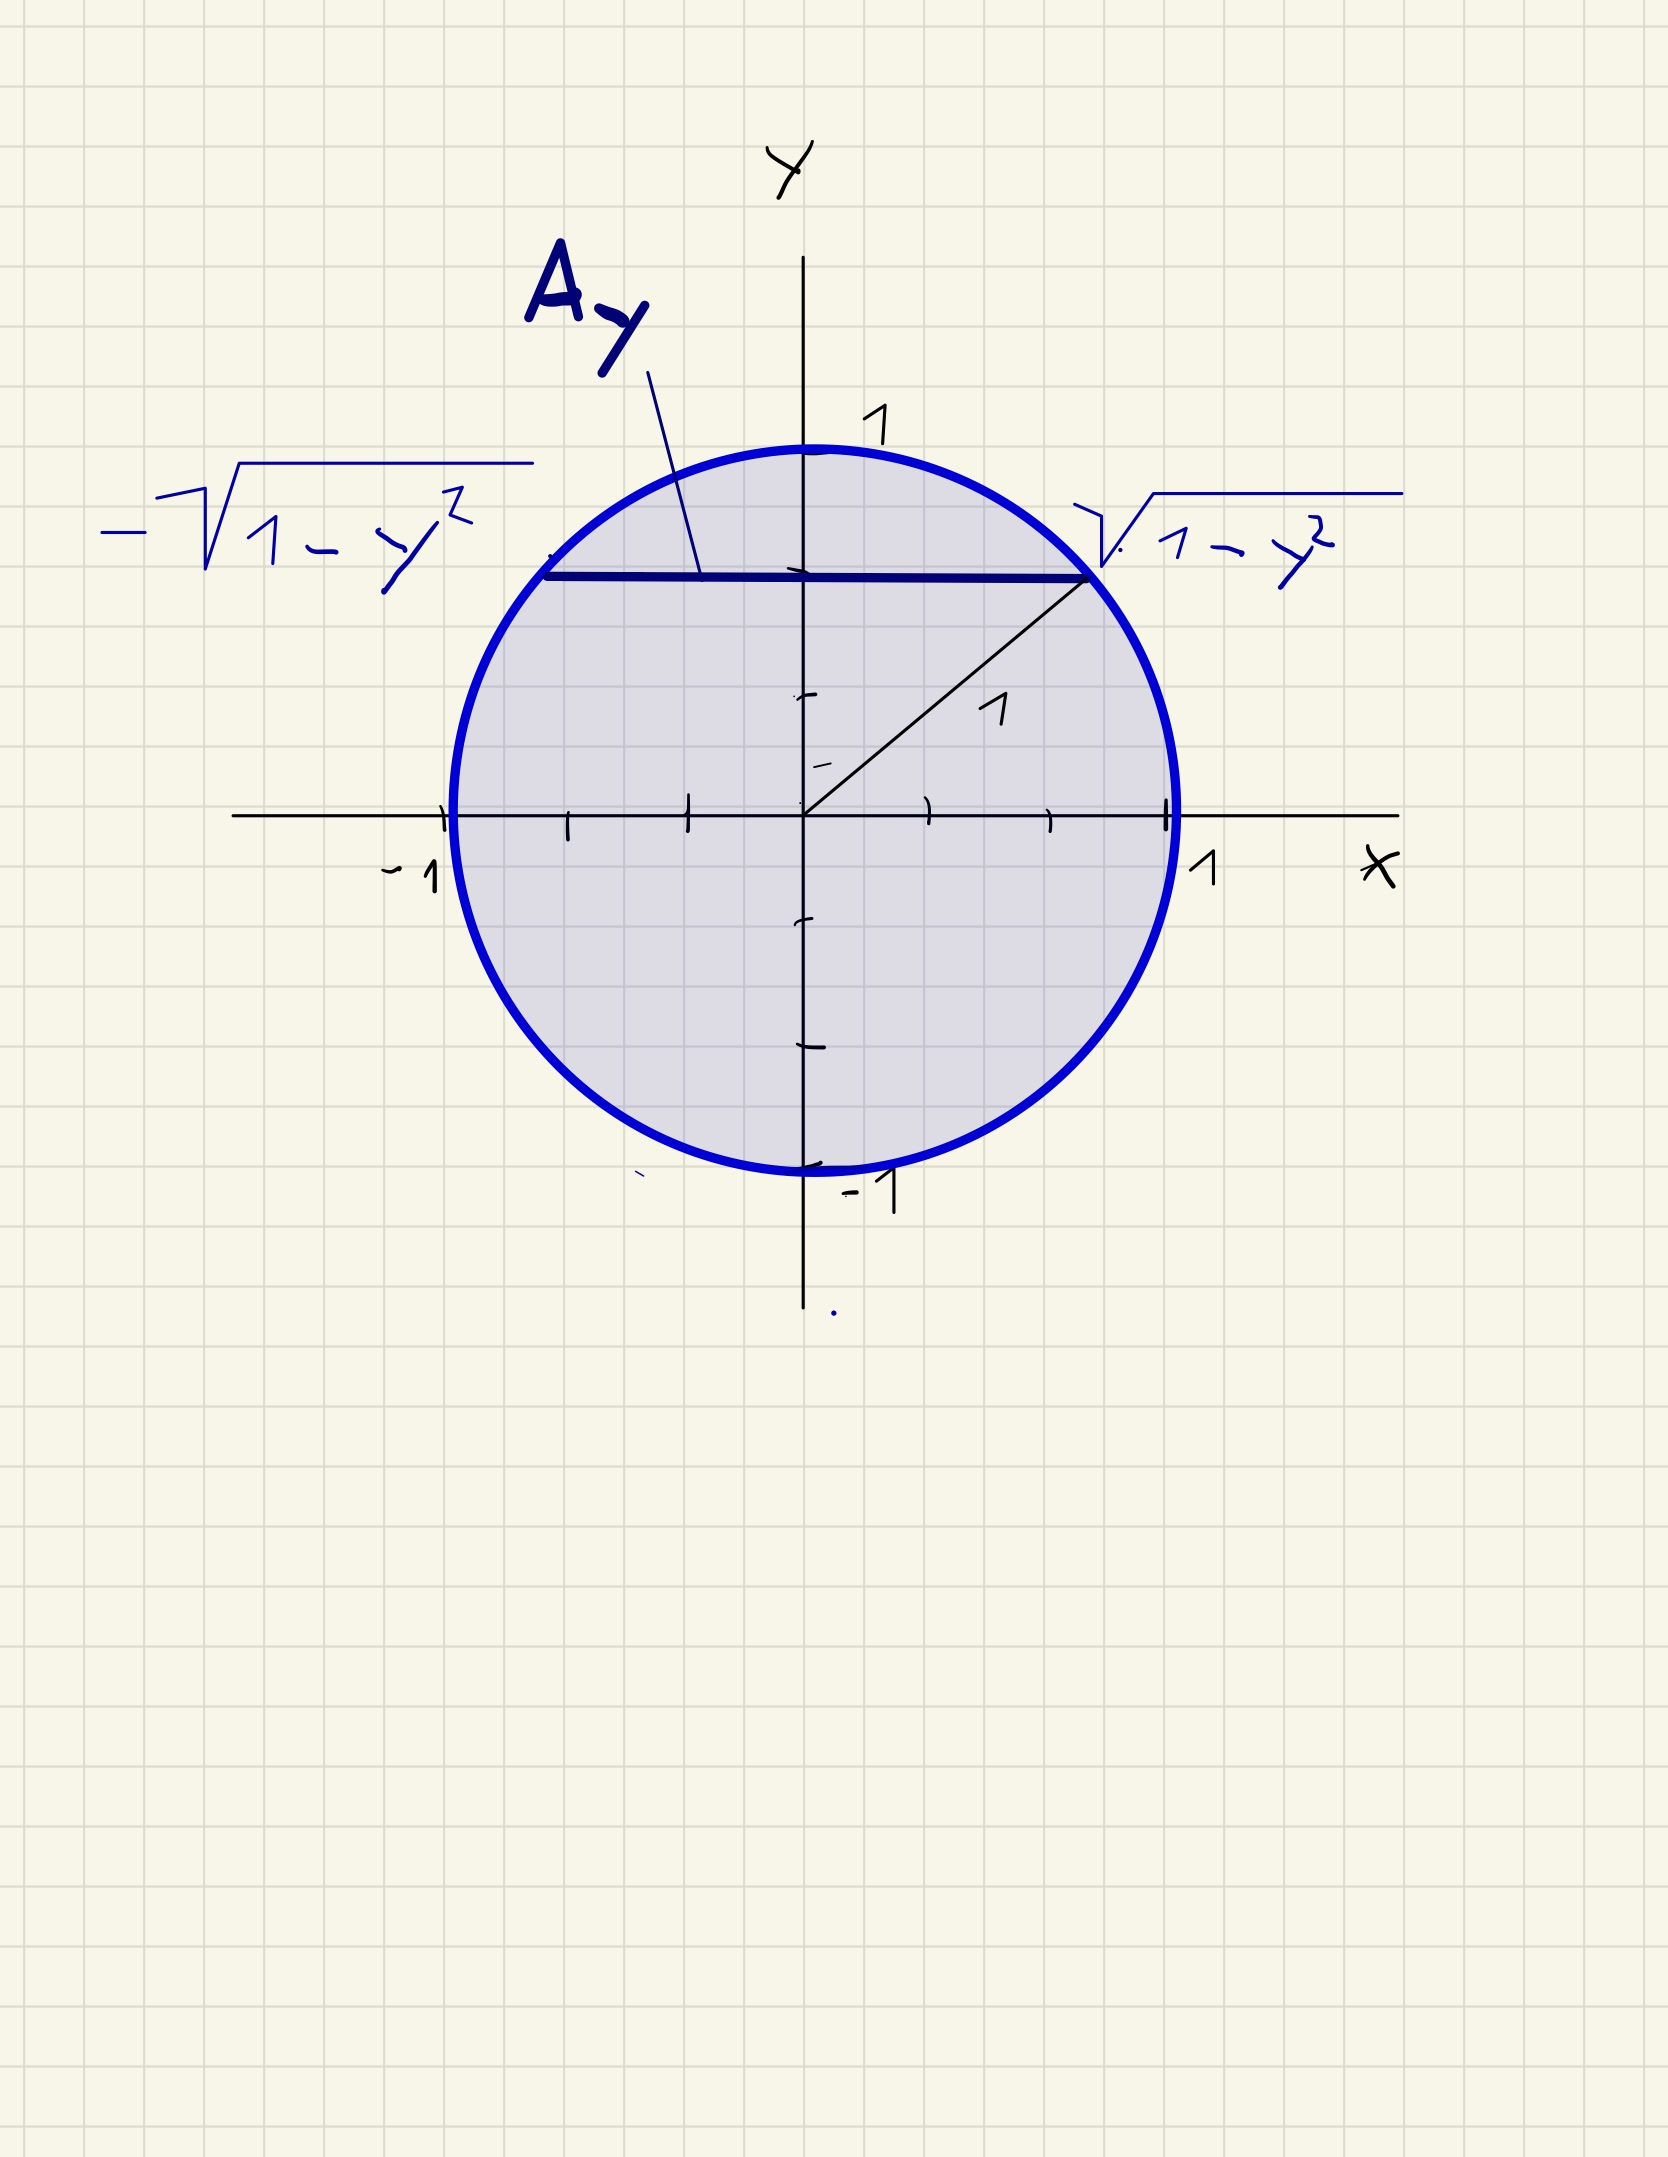
\includegraphics[width=0.8\textwidth]{images/Kreis}
\end{figure}
 \end{frame}



\begin{frame}
    \frametitle{Angewandte Mathematik}
\framesubtitle{Lebesgue Integral}
\begin{block}{Quader und lineare Abbildungen}
Seien $U$ und $V$ offene Teilmengen des $\mathbb{R}^n$, $T': U \to V$ ein lineare Abbildung und  $Q \in \mathbb{I}(n)$ ein Quader.
Dann gilt:
 $$ \text{vol}  (T'(Q))   =  \det (T') \cdot   \text{vol}(Q) \; .$$
\end{block}
 \end{frame}

\begin{frame}
    \frametitle{Angewandte Mathematik}
\framesubtitle{Beweis}
Für Vektoren $a_1, \cdots a_n$ im $\mathbb{R}^n$ heißt die Menge 
$$ P(a_1, \cdots,  a_n) := \biggl \{  x = \sum_{k=1}^n t_k a_k  \; | \; t_1, \cdots , t_n \in [0,1]  \biggr \}$$
Parallelotop.
\begin{figure}[H]
      \centering
    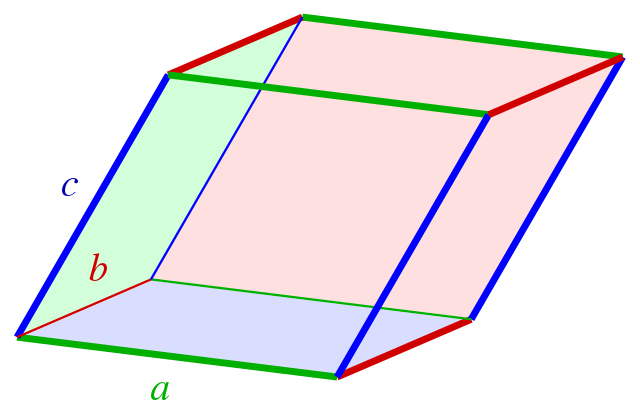
\includegraphics[width=0.6 \textwidth]{images/640px-Parallelepiped-0}    
\end{figure}
 \end{frame}

\begin{frame}
    \frametitle{Angewandte Mathematik}
\framesubtitle{Beweis}

Es gilt  $$  \text{vol} \bigr( P(a_1, \cdots, a_n) \bigr) =  | det (a_1, \cdots, a_n) |   \; .$$

\href{https://www.math.uchicago.edu/~may/VIGRE/VIGRE2007/REUPapers/FINALAPP/Peng.pdf}{Ausfürlicher Beweis}
 \end{frame}



\begin{frame}
    \frametitle{Angewandte Mathematik}
\framesubtitle{Lebesgue Integral}
\begin{block}{Diffeomorphismus}
Seien $U$ und $V$ offene Teilmengen des $\mathbb{R}^n$. Eine Abbildung  $T: U \to V$ heißt Diffeomorphismus, wenn eine  Umkehrfunktion $T^{-1}: V  \to U$ existiert, also $T^{-1} (T (u)) = u$ gilt für alle $u \in U$, die ebenfalls differenzierbar ist.
\end{block}

\begin{block}{}
Für eine invertierbare Matrix $A$ ist $T(x):= Ax$ ein Diffeomorphismus.
\end{block}
 \end{frame}


\begin{frame}
    \frametitle{Angewandte Mathematik}
\framesubtitle{Lebesgue Integral}
\begin{block}{Transformationssatz}
Seien $U$ und $V$ offene Teilmengen des $\mathbb{R}^n$, $T: U \to V$ ein Diffeomorphismus und $f: V \to \mathbb{R}$ eine integrierbare Funktion. Dann gilt:
$$ \int_V  f(y)  d \mu = \int_U f(T (x))  \cdot | \det(T' (x)) | d \mu   \; .$$
\end{block}
 \end{frame}

\begin{frame}
    \frametitle{Angewandte Mathematik}
\framesubtitle{Beweis}
Seien $I_k \in \mathbb{I}(n)$ Quader, $J_k := T(I_k)$ und $b_k = T(c_k)$. Dann ist 
$$\sum_{k=1}^n  b_k  \text{vol}(J_k) \approx  \sum_{k=1}^n T(c_k) \cdot | \det T' (c_k)|  \text{vol}(I_k) \; .$$
Die Behauptung folgt dann (nicht trivial) durch den Übergang zu Grenzwerten mit entsprechenden Konvergenzsätzen.
 \end{frame}


\begin{frame}
    \frametitle{Angewandte Mathematik}
\framesubtitle{Lebesgue Integral}
\begin{block}{Beispiel}
Wir betrachten den Ball $B_r^3(0):= \{ x \in \mathbb{R}^3 \; | \; || x || \leq r  \}$, den Quader $I := [0,r] \times [- \pi, \pi] \times [- \frac{\pi}{2}, \frac{\pi}{2}]$ und die Abbildung
\begin{align*}
T : I \to B_1^3(0) \\
T(r, \varphi, \psi) := \begin{pmatrix} r \cos(\varphi) \cos(\psi)   \\  r \sin(\varphi) \cos(\psi) \\ r  \sin(\psi)     \end{pmatrix}
\end{align*}
\end{block}
\begin{block}{Beispiel}
$\det T'(r, \varphi, \psi) = r^2 \cos(\psi)$
\end{block}
 \end{frame}

\begin{frame}
    \frametitle{Angewandte Mathematik}
\framesubtitle{Lebesgue Integral}
\begin{align*}
\int_{B_r^3(0)} 1 d\mu = \int_{ [0,r] } \int_{ [- \pi, \pi]} \int_{[- \frac{\pi}{2}, \frac{\pi}{2}]} r^2 \cos(\psi) d \psi \; d \varphi \; dr = \frac{4} {3} \pi r^3
\end{align*}
\begin{figure}[H]
      \centering
    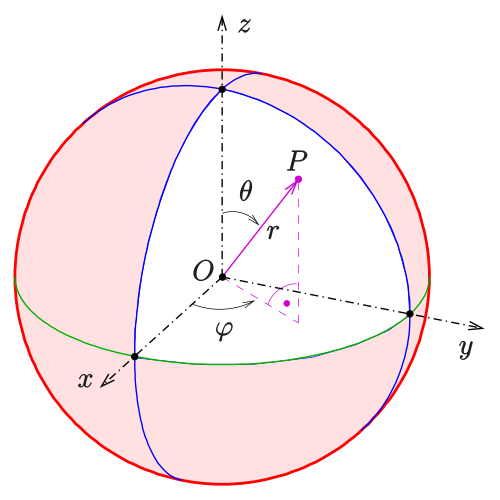
\includegraphics[width=0.4 \textwidth]{images/500px-Kugelkoord-def}    
\end{figure}
 \end{frame}



\begin{frame}
    \frametitle{Angewandte Mathematik}
\framesubtitle{Lebesgue Integral}
\begin{block}{Konvergenz fast überall}
Eine Folge von Funktionen $f_k$ konvergiert Punktweise fast überall gegen eine Funktion $f$, falls es eine Nullmenge $N$ gibt, mit 
$\lim_{k \to \infty} f_k (x) = f(x)$ für alle $x \in \mathbb{R}^n \setminus N$.
\end{block}
 \end{frame}


\begin{frame}
    \frametitle{Angewandte Mathematik}
\framesubtitle{Lebesgue Integral}
\begin{block}{Satz von Lebesgue}
Sei $f_k$ eine Folge integrierbarer Funktionen auf $\mathbb{R}^n$ die fast überall Punktweise gegen eine Funktion $f$ konvergiert.
Es gebe eine integrierbare Funktion $F$ mit $|f_k (x)| \leq F(x) $ für alle $x \in \mathbb{R}^n$ und alles $k$. Dann ist $f$ integrierbar und es gilt
$$ \int f(x) d \mu = \lim_{k \to \infty} \int f_k(x) d \mu $$
\end{block}
 \end{frame}



\begin{frame}
    \frametitle{Angewandte Mathematik}
\framesubtitle{Lebesgue Integral}
\begin{block}{Parameterabhängige Integrale}
Sei $f: X \times T \subset \mathbb{R}^{n-p} \times \mathbb{R}^p$ eine Funktion, so dass für festes $x \in X$ die Funktion $f_x(t) := f(x,t)$ über $T$ integrierbar ist. Durch Integration erhält man die Funktion 
$$ F(x) := \int_T f(x,t)  d \mu_T$$ 
auf $X$.
\end{block}
 \end{frame}


\begin{frame}
    \frametitle{Angewandte Mathematik}
\framesubtitle{Lebesgue Integral}
\begin{block}{Stetigkeitssatz}
$f$ habe zusätzlich die Eigenschaften:
\begin{itemize}
\item Für festes $t$ ist $f_t(x):= f(x,t)$ stetig.
\item Es gibt auf $T$ eine integrierbare Funktion $\phi$ mit $\phi(t) \geq 0$ und $|f(x,t)| \leq \phi(t)$ für alle $(x,t) \in X \times T$.
\end{itemize}
Dann ist die oben definierte Funktion $F$ stetig. 
\end{block}
 \end{frame}


\begin{frame}
    \frametitle{Angewandte Mathematik}
\framesubtitle{Beweis}
Sei  $x_k \to x$   eine konvergente Folge in $X$ und $f_k(t):= f(x_k,t)$. Nach Voraussetzung konvergiert diese Folge punktweise gegen die Funktion $f_x(t)$ und $| f_k (x) | \leq \phi(x)$. Mit dem Satz von Lebesgue folgt
$$ \lim_{k \to \infty} \int_T f_k(t) d \mu_T = \int_T f(x,t) d \mu_T$$
und damit $ \lim_{k \to \infty} F(x_k) =  F(x)$.
 \end{frame}

\begin{frame}
    \frametitle{Angewandte Mathematik}
\framesubtitle{Lebesgue Integral}
\begin{block}{Differentiationssatz}
$f$ habe zusätzlich die Eigenschaften:
\begin{itemize}
\item Für festes $t$ ist $f_t(x):= f(x,t)$ stetig differenzierbar.
\item Es gibt auf $T$ eine integrierbare Funktion $\phi$ mit $\phi(t) \geq 0$ und $| \frac{\partial}{\partial x_i} f(x,t)| \leq \phi(t)$ für alle $(x,t) \in X \times T$ und $i=1, \cdots n-p$.
\end{itemize}
Dann ist die oben definierte Funktion $F$ stetig differenzierbar und es gilt
$$\frac{\partial}{\partial x_i} F(x)  = \int_T \frac{\partial}{\partial x_i} f(x,t) d \mu_T \; .$$ 
\end{block}
 \end{frame}

\begin{frame}
    \frametitle{Angewandte Mathematik}
\framesubtitle{Beweis}
Sei $x_k := x_0 + h_k e_i$ und 
$$ \varphi_k (t) := \frac{f(x_k,t)  - f(x_0,t)  }{h_k} \; .$$
Damit sind die Funktionen  $\varphi_k $ integrierbar und für jedes $t \in T$ gilt

$$  \lim_{k \to \infty} \varphi_k (t) = \frac{\partial}{\partial x_i}f(x_0, t) \; .$$
Mit dem Satz von Lebesgue gilt
$$ \lim_{k \to \infty}  \int_T \varphi_k (t) d \mu_T = \int_T   \frac{\partial}{\partial x_i}f(x_0, t) d \mu_T $$
und da 
$$  \int_T \varphi_k (t) d \mu_T = \frac{F(x_k) -F(x_0)}{h_k}$$ ist, folgt die Behauptung.
 \end{frame}



\begin{frame}
    \frametitle{Angewandte Mathematik}
\framesubtitle{Lebesgue Integral}
\begin{block}{Faltung}
Für integrierbare Funktionen  $f$ und $g$ auf $\mathbb{R}^n$ ist die Faltung definiert durch
\begin{align}
(f * g )(x) := \int_{\mathbb{R}^n}  f(y) \cdot g(x-y) \; d \mu_y  \; .
\end{align}
Das Integral existiert wegen dem Satz von Fubini.
\end{block}
 \end{frame}





\begin{frame}
    \frametitle{Angewandte Mathematik}
\framesubtitle{Lebesgue Integral}
\begin{block}{Ableitung einer Faltung}
Für die Faltung gilt bei entsprechenden Voraussetzungen der Differenzierbarkeit der Funktionen 
$$ \partial^{\alpha} (f  * g) = f * \partial^{\alpha} g \; .$$
\end{block}
 \end{frame}





\begin{frame}
    \frametitle{Digitale Bilder}
\framesubtitle{}
    \begin{block}{Umwandlung von Bildern}
\begin{itemize}
\item Viele Verfahren der  Signalverarbeitung haben ihren Ursprung in der Analysis. Um diese anwenden zu können, müssen diskrete Daten  in kontinuierliche Daten umgewandelt werden.
\item Auf der anderen Seite kann  ein Computer nur diskrete Daten  verarbeitet. Kontinuierliche Signale (zum Beispiel von Sensoren) müssen daher in diskrete Daten umgewandelt werden.
\end{itemize}
\end{block}

 \end{frame}

\begin{frame}
    \frametitle{Digitale Bilder}
\framesubtitle{}

   \begin{block}{Diskretes Bild}
Ein $n$ dimensionales diskretes Bild ist eine Abbildung 
\begin{align*}
U : [1, \ldots, N_1] \times   \cdots \times [1, \ldots, N_n]   \to R
\end{align*}
von $n$ diskreten Intervallen  $[1, \ldots, N_k]  \subset \mathbb{N}$  in einen Farbraum $R$.
\end{block}

   \begin{block}{Kontinuierliches Bild}
Ein $n$ dimensionales kontinuierliches Bild ist eine Abbildung 
\begin{align*}
u : I_1 \times   \cdots \times I_n   \to R
\end{align*}
von $n$ reellen Intervallen $I_k \subset \mathbb{R}$ in einen Farbraum $R$.
\end{block}

 \end{frame}


\begin{frame}
    \frametitle{Digitale Bilder}
\framesubtitle{}
\begin{block}{Abtastung}
Für ein kontinuierliches  Bild $u : I^n \to R$ erhält man durch gewichtete Mittelungen
$U_i := \int_{I^n} \phi (x) u(x - x_i) dx$ ein diskretes Bild. 
\end{block}
 \end{frame}

\begin{frame}
    \frametitle{Digitale Bilder}
\framesubtitle{}
    \begin{block}{}
Für ein eindimensionales, diskretes Bild $U : [1, \ldots, N]  \to R$ bezeichne  $U_{j} := U(j)$.
\end{block}
    \begin{block}{Stückweise konstante Interpolation}
Definiere $\phi^0 (x) : = 1_{ [-\frac{1} {2} ,  \frac{1} {2}) }(x) : =\begin{cases}
   1 , & \text{für } -\frac{1} {2}  \leq x < \frac{1} {2}  \\
    0  & \text{sonst } 
  \end{cases} $, $\phi^0_j(x):= \phi^0 (x - j)$ und
 $u(x) := \sum_{j=1}^{N} U_j \phi^0_j(x)$ 
\end{block}

 \end{frame}





\begin{frame}
    \frametitle{Digitale Bilder}
\framesubtitle{}
\begin{block}{Höherdimensionale stückweise  Interpolation}
Für ein 2-dimensionales, diskretes Bild $U : [1, \ldots, N] \times   [1, \ldots, M] \to R$ definiere 
 $u(x, y) := \sum_{i=1}^{N} \sum_{j=1}^{M}  U_{i,j} \cdot \phi_i(x) \cdot \phi_j(y)$ und analog für n-dimensonale Bilder....
\end{block}
 \end{frame}


\begin{frame}
    \frametitle{Digitale Bilder}
\framesubtitle{}
\begin{block}{Abtastung}
Für ein kontinuierliches  Bild $u : I^n \to R$ erhält man durch gewichtete Mittelungen
$U_i := \int_{I^n} \phi (x - x_i) u(x) dx$ ein diskretes Bild. 
\end{block}
 \end{frame}



\begin{frame}
    \frametitle{Diskrete Faltung}
\framesubtitle{}

    \begin{block}{Diskrete Faltung}
Für zwei diskrete  Funktionen $U : [1, \ldots, N]  \to R$ und $H : [1, \ldots, N]  \to R$ mit stückweisen konstanten Interpolation $u(x) := \sum_{l=1}^{N} U_l \phi^0_j(x)$ und 
$h(x) := \sum_{m=1}^{N} H_m \phi^0_m(x)$ ergibt die Faltung 
\begin{align*}
& (h * u)(k) = \int u(y)h(k-y)  \; dy \\
& = \int \ \sum_{l=1}^{N} U_l \phi^0(y-l) \sum_{m=1}^{N} H_m \phi^0(k-y-m) \\
& = \sum_{l=1}^{N}   \sum_{m=1}^{N} U_l  H_m  \int  \phi^0(y-l) \phi^0(k-y-m) \; dy 
\end{align*}

\end{block}
 \end{frame}

\begin{frame}
    \frametitle{Diskrete Faltung}
\framesubtitle{}

    \begin{block}{Diskrete Faltung}
Da für das Integral 
\begin{align*}
  \int  \phi^0(y-l) \phi^0(k-y-m)  \; dy  = \begin{cases}
1 \text{ falls } m = k -l\\
0 \text{ sonst }
\end{cases}
\end{align*}
gilt, folgt die Darstellung
\begin{align*}
 (u  * h)(k) = \sum_l U_l H_{k-l}
\end{align*}

\end{block}

 \end{frame}


\begin{frame}
    \frametitle{Kantenerkennung}
\framesubtitle{}
\begin{block}{Kanten}
Kanten sind durch schnelle Änderungen des Farbwertes gekennzeichnet. Sie sind damit Extremstellen der ersten Ableitung.
\end{block}
\begin{figure}[htp]
      \centering
Intensität und Gradient entlang eines Bildschnittes \\
    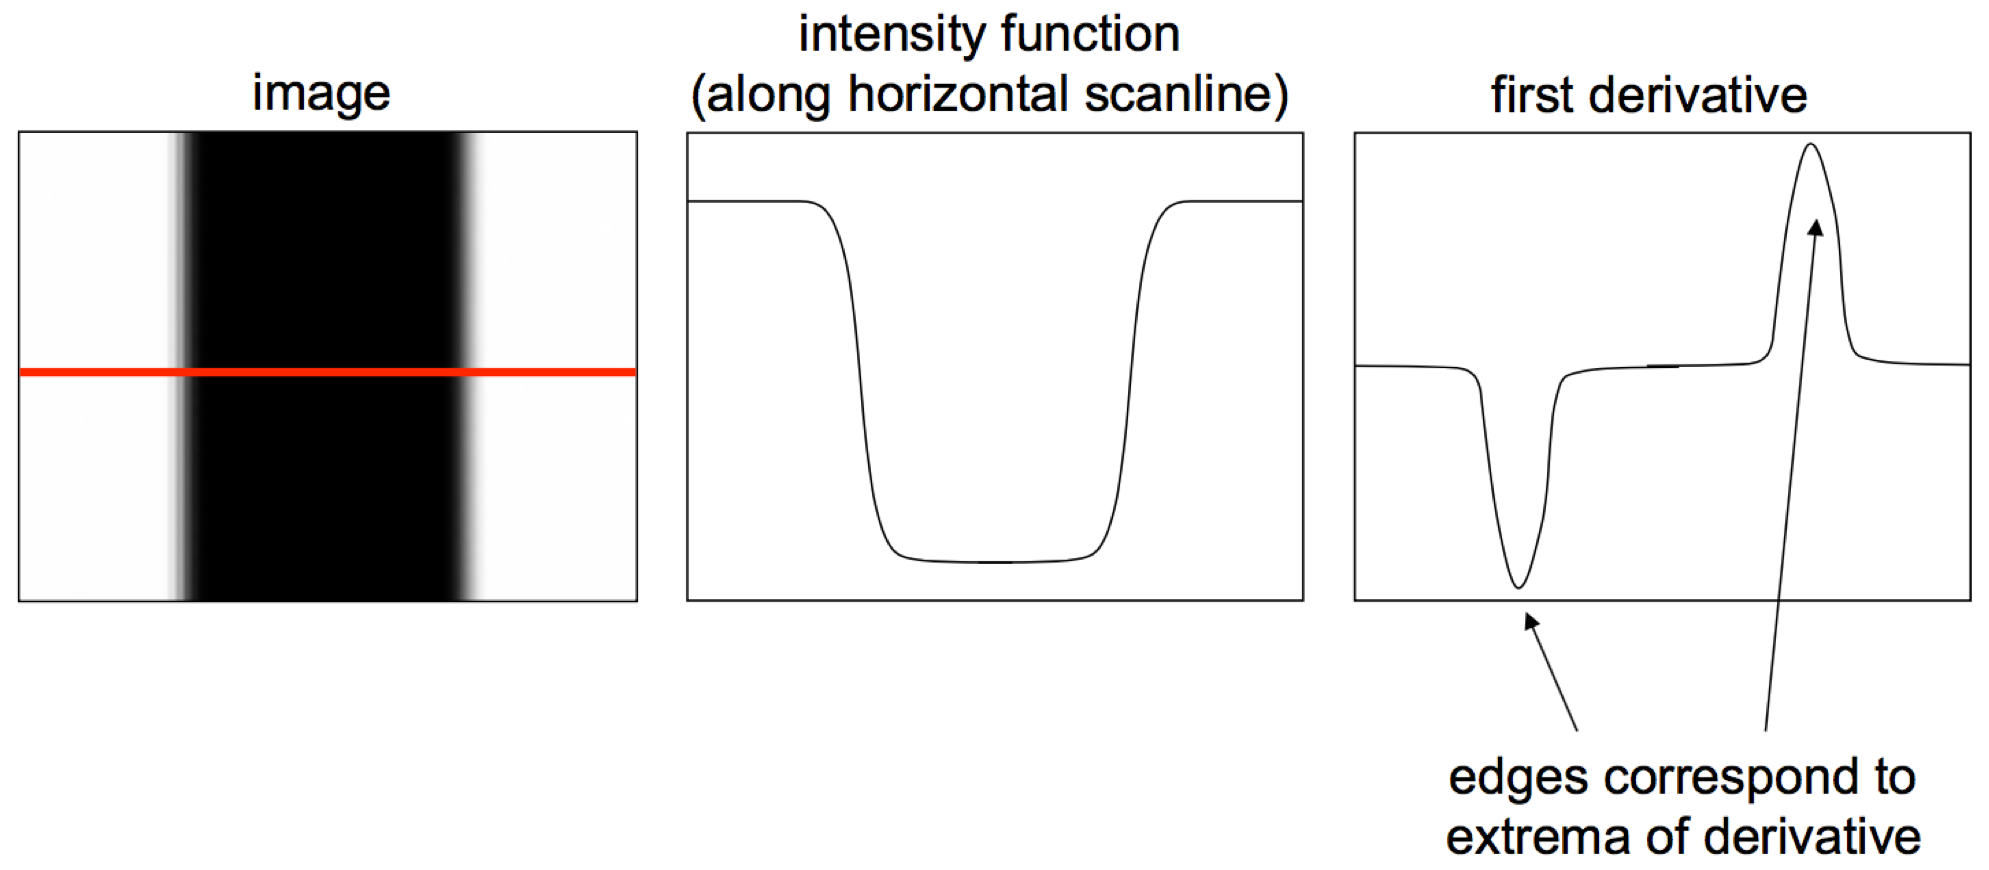
\includegraphics[width=0.65\textwidth]{images/edgedetection} 
      \caption{Quelle: ai.stanford.edu}
\end{figure}

 \end{frame}

\begin{frame}
    \frametitle{Kantenerkennung}
\framesubtitle{}
\begin{block}{Gradientenbasierte Kantenerkennung}
Bei der Detektion von Kanten mit Hilfe des Gradienten ist   Rauschen ein Problem, da sich  hier ebenfalls  der Farbwert schnell ändert. 
\end{block}
\begin{figure}[htp]
      \centering
Rauschen \\
    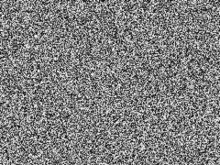
\includegraphics[width=0.45\textwidth]{images/noise} 
      \caption{Quelle: Wikipedia}
\end{figure}

 \end{frame}

\begin{frame}
    \frametitle{Kantenerkennung}
\framesubtitle{}
\begin{block}{Gradientenbasierte Kantenerkennung}
Idee: Wende einen Filter an, der das Rauschen reduziert und bilde dann den Gradienten. Bilde also den Gradienten
\begin{align*}
\frac{\partial (u * f)(x)}{\partial x} 
\end{align*}
wobei $f$ ein Faltungskern ist.
\end{block}

\begin{block}{Ableitung von Faltungen}
Es gilt
\begin{align*}
\frac{\partial (u * f)(x)}{\partial x} = (u * f')(x)
\end{align*}

\end{block}

 \end{frame}


\begin{frame}
    \frametitle{Kantenerkennung}
\framesubtitle{}
\begin{block}{Gradientenbasierte Kantenerkennung}
Welcher Filter ist gut geeignet?
\end{block}
\begin{block}{Kantenerkennung nach Canny}
Es gibt Kanten auf unterschiedlichen Skalen ("grobe Kanten" und "feine Kanten"). Wähle daher einen parameterabhängigen Faltungskern
$f_\sigma$. Zu einem Originalbild $u_0$ bekommen wir eine ganze Klasse von Bildern
\begin{align*}
u(x, \sigma) = u_0 * f_\sigma(x) \;.
\end{align*}
 \end{block}

 \end{frame}

\begin{frame}
    \frametitle{Kantenerkennung}
\framesubtitle{}

\begin{block}{Kantenerkennung nach Canny}
Die Stellen der Kanten soll sich bei wachsendem $\sigma$ nicht verändern und ebenso sollen auch keine Kanten hinzukommen. 
Deswegen soll in einem Kantenpunkt $x_0$ von $u_0$ gelten:
\begin{align*}
\frac{\partial^2}{\partial x^2} > 0 \Rightarrow \frac{\partial}{\partial \sigma}  u(x_0, \sigma) > 0 \\
\frac{\partial^2}{\partial x^2} = 0 \Rightarrow \frac{\partial}{\partial \sigma}  u(x_0, \sigma) = 0 \\
\frac{\partial^2}{\partial x^2} < 0 \Rightarrow \frac{\partial}{\partial \sigma}  u(x_0, \sigma) <0
\end{align*}
 \end{block}

 \end{frame}

\begin{frame}
    \frametitle{Kantenerkennung}
\framesubtitle{}

\begin{block}{Kantenerkennung nach Canny}
Für einen allgemeinen Punkt soll daher gelten:
\begin{align*}
&\frac{\partial^2}{\partial x^2}  u(x, \sigma)  =  \ \frac{\partial}{\partial \sigma}  u(x, \sigma)  \\
&  u(x, 0) = u_0(x) 
\end{align*}
 \end{block}

\begin{block}{Kantenerkennung nach Canny}
Diese partielle Differentialgleichung hat die eindeutige Lösung
\begin{align*}
&  u(x, \sigma) = (u_0 * G^{\sqrt{2\sigma}}) (x)
\end{align*}
wobei $ G^{\sqrt{2\sigma}}$ der Gaußfilter ist.
 \end{block}

 \end{frame}


\begin{frame}
    \frametitle{Kantenerkennung}
\framesubtitle{}

\begin{block}{Kantenerkennung nach Canny}
Die Kantenerkennung nach Canny faltet ein gegebenes Bild $u$ zuerst mit einem Gaußkernel $G^{\sigma}$. Danach wird  der Betrag der Ableitung und seine Richtung berechnet: 
\begin{align*}
p(x) = & || \nabla (u * G^\sigma)(x) || \\
&= \sqrt{ (\frac{\partial}{\partial x_1} (u * G^\sigma)(x))^2 + (\frac{\partial}{\partial x_2} (u * G^\sigma)(x))^2 } \\
\theta(x) & = \angle  \nabla (u * G^\sigma)(x) = \arctan \biggl( \frac{\frac{\partial}{\partial x_2} (u * G^\sigma)(x)}{\frac{\partial}{\partial x_1} (u * G^\sigma)(x)} \biggr)
\end{align*}


 \end{block}

 \end{frame}



\begin{frame}
    \frametitle{Kantenerkennung}
\framesubtitle{}
\begin{block}{Kantenerkennung nach Canny}
Als Kanten werden lokale Maxima von $p(x)$ in Richtung $(\sin \theta(x), \cos \theta(x)  )$
\end{block}
\begin{figure}[htp]
      \centering
Kanten als lokale Maxima in Kantenrichtung \\
    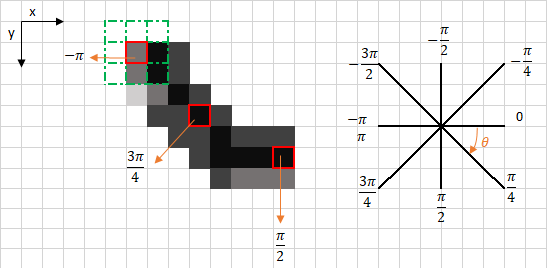
\includegraphics[width=0.55\textwidth]{images/canny_max} 
      \caption{Quelle: towardsdatascience.com}
\end{figure}

 \end{frame}




\begin{frame}
    \frametitle{Kantenerkennung}
\framesubtitle{}
\begin{block}{Kantenschärfen mit Laplace}
Durch die Operation $u - \tau \bigtriangleup u$ werden die Kanten hervorgehoben.
\end{block}
\begin{figure}[htp]
      \centering
Kanten als lokale Maxima in Kantenrichtung \\
    \includegraphics[width=0.55\textwidth]{images/laplace1} \\
    \includegraphics[width=0.35\textwidth]{images/laplace2} 
      \caption{Quelle:OpenCV}
\end{figure}
 \end{frame}

\begin{frame}
    \frametitle{Kantenerkennung}
\framesubtitle{}
\begin{figure}[htp]
      \centering
Kantenschärfung \\
    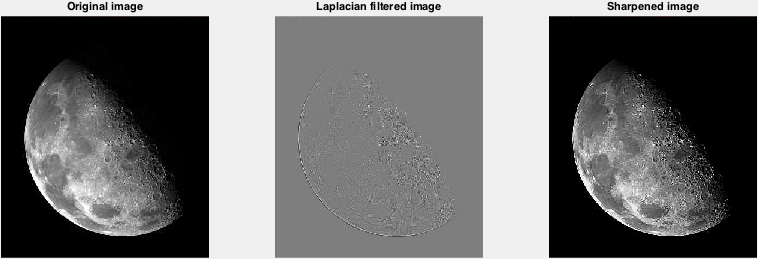
\includegraphics[width=0.95\textwidth]{images/sharpening} 
      \caption{Quelle: Stackoverflow}
\end{figure}
 \end{frame}





\begin{frame}
    \frametitle{Kantenerkennung}
\framesubtitle{}
\begin{block}{}
\end{block}
 \end{frame}

\end{document}

